\subsection{Optical Encoding of Spin Variables}
The core principle of the Spatial Photonic Ising Machine depends on mapping discrete spin variables $\sigma_i$ to the continuous phase degrees of freedom of an electromagnetic wave. We utilize a Spatial Light Modulator (SLM) to impose a phase shift $\phi_j$ on an incident coherent beam at pixel $j$. The mapping is binary:

\begin{equation}
\sigma_j = \begin{cases} 
+1 & \text{if } \phi_j = 0 \\
-1 & \text{if } \phi_j = \pi
\end{cases}
\end{equation}

Considering the finite aperture of each pixel, the electric field contribution from the $j$-th spin at the SLM plane can be modeled as a rectangular function. In the Fourier domain, this corresponds to a Sinc function. The total electric field $E(\mathbf{x})$ at the detection plane (Fourier plane) is given by the superposition of contributions from all $N$ pixels:

\begin{equation}
E(\mathbf{x}) \propto \sum_{j=1}^{N} \xi_j \sigma_j e^{i \mathbf{k}_j \cdot \mathbf{x}} \text{sinc}(W(\mathbf{x} - \mathbf{x}_j))
\end{equation}

where $\xi_j$ is the amplitude uniformity factor and $\mathbf{k}_j$ is the wavevector associated with pixel $j$.

\begin{figure}[h]
    \centering
    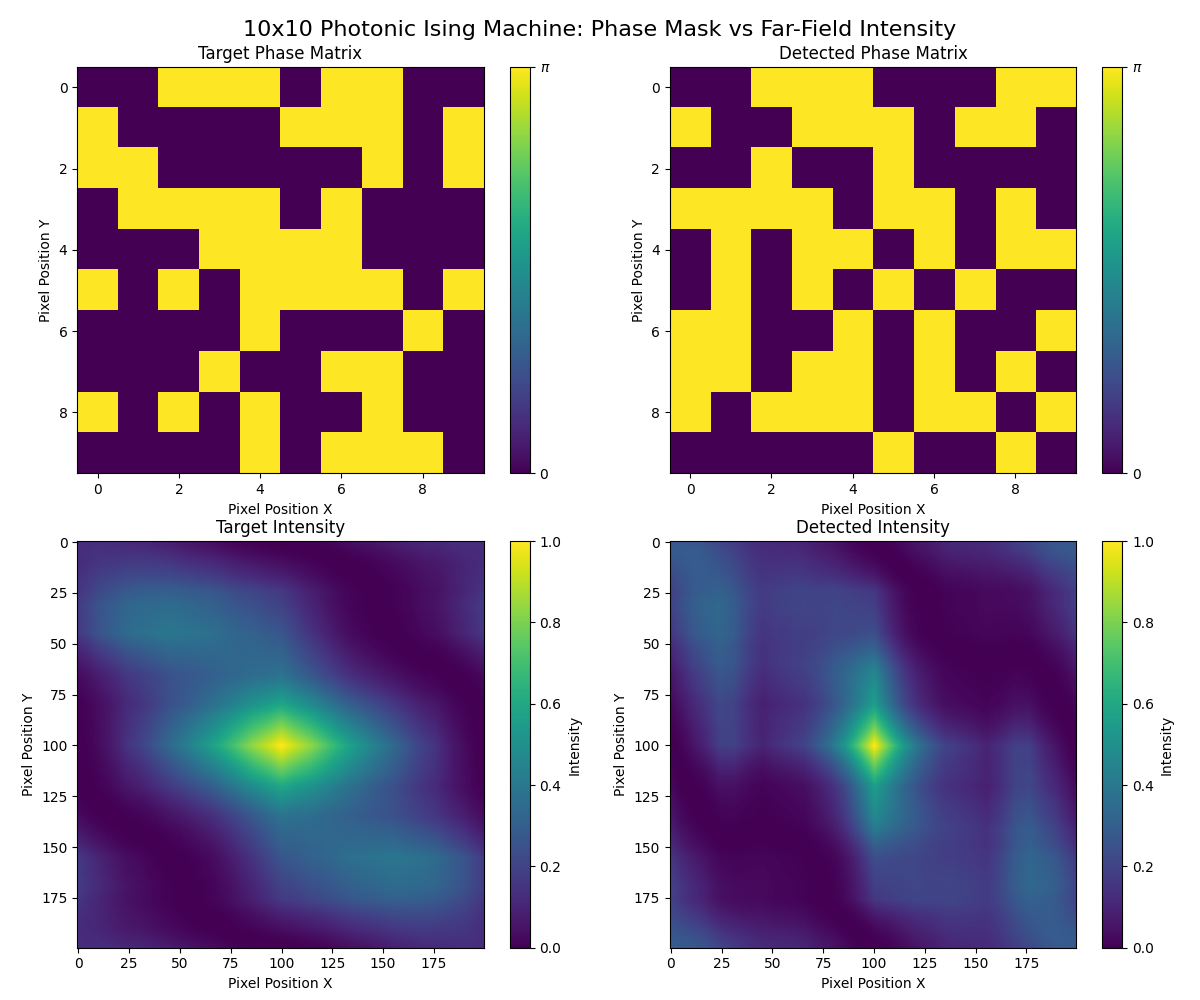
\includegraphics[width=0.45\textwidth]{../../docs/simulation_result.png}
    \caption{Visual demonstration of the Spatial Photonic Ising Machine. Left: The phase mask displayed on the SLM, representing the spin configuration. Right: The resulting far-field intensity pattern $I(\mathbf{x})$, which physically computes the Hamiltonian energy via optical interference. The speckle pattern acts as the energy landscape for the optimization process.}
    \label{fig:simulation_result}
\end{figure}

\subsection{Hamiltonian Engineering via Interference}
The "computation" in this photonic system occurs naturally through optical interference. The intensity $I(\mathbf{x})$ measured by the CCD camera is the square of the electric field modulus: $I(\mathbf{x}) = |E(\mathbf{x})|^2$. Expanding this reveals the interaction terms:

\begin{equation}
I(\mathbf{x}) = \sum_{j,h} \xi_j \xi_h \sigma_j \sigma_h K_{jh}(\mathbf{x})
\end{equation}

where $K_{jh}(\mathbf{x})$ is the interference kernel dependent on the relative positions of pixels $j$ and $h$. This expressions effectively reconstructs an Ising-like energy landscape. By measuring the difference between the detected intensity pattern and a target intensity pattern $I_T(\mathbf{x})$ (which encodes the specific problem constraints), we can define an optical cost function:

\begin{equation}
f = \int |I(\mathbf{x}) - I_T(\mathbf{x})|^2 d\mathbf{x}
\end{equation}

Minimizing this cost function effectively drives the system toward the ground state of the encoded Ising Hamiltonian. The optimization process is implemented using a feedback loop in the digital domain, specifically a \textbf{Metropolis-Hastings} algorithm with \textbf{Cluster Updates}.

\subsection{Algorithm and Feedback Loop}
The system operates as an optical-digital hybrid solver. The workflow for finding the ground state is as follows:

\begin{enumerate}
    \item \textbf{Initialization}: A random phase mask $\phi(\mathbf{x})$ is generated on the SLM, corresponding to a random spin configuration $\sigma$.
    \item \textbf{Optical Evolution}: The laser beam diffracts through the SLM, and the interference pattern $I(\mathbf{x})$ is captured by the camera at the Fourier plane.
    \item \textbf{Cost Evaluation}: The digital processor computes the energy $E = \int |I(\mathbf{x}) - I_T(\mathbf{x})|^2 d\mathbf{x}$.
    \item \textbf{Cluster Update}: To escape local minima, we employ a cluster update strategy (similar to the Wolff algorithm). A cluster of spins is flipped simultaneously rather than a single spin. The cluster size scales logarithmically with iteration count.
    \item \textbf{Acceptance Criterion}: The new configuration is accepted with probability $P = \min(1, e^{-\Delta E / T})$, where $T$ is an adaptive temperature parameter that decreases over time (Simulated Annealing).
\end{enumerate}

This approach allows the system to traverse the energy landscape efficiently, avoiding the "critical slowing down" typical of local update rules near phase transitions.

\subsection{Mattis Spin Glass Implementation}
A key advantage of this architecture is the flexibility to implement complex Hamiltonians such as the \textbf{Mattis Spin Glass}. By modulating the amplitude $\xi_j$ of the incident light at each pixel (in addition to the phase), we can engineer specific coupling matrices $J_{jh} = \xi_j \xi_h$. 
Specifically, if $\xi_j$ is drawn from a binary distribution $\{+1, -1\}$, the system simulates a randomness-induced frustration that characterizes spin glasses. The degree of correlation between the final spin state $\sigma$ and the amplitude mask $\xi$ (Spin-$\xi$ Correlation) serves as an order parameter to verify ground state retrieval:
\begin{equation}
C = \frac{1}{N} \sum_j \sigma_j \xi_j
\end{equation}
A value of $|C| \approx 1$ indicates successful solving of the Mattis model.

\subsection{Simulation Parameters}
To validate the theoretical framework, we performed high-fidelity numerical simulations using the parameters of a typical commercial experimental setup:
\begin{itemize}
    \item \textbf{Wavelength ($\lambda$)}: 532 nm (Green Laser)
    \item \textbf{Focal Length ($f$)}: 500 mm
    \item \textbf{Pixel Pitch ($p$)}: 20 $\mu$m (Standard LCOS-SLM)
    \item \textbf{System Size ($N$)}: $10^2$ to $100^2$ spins
\end{itemize}

\begin{figure}[h]
    \centering
    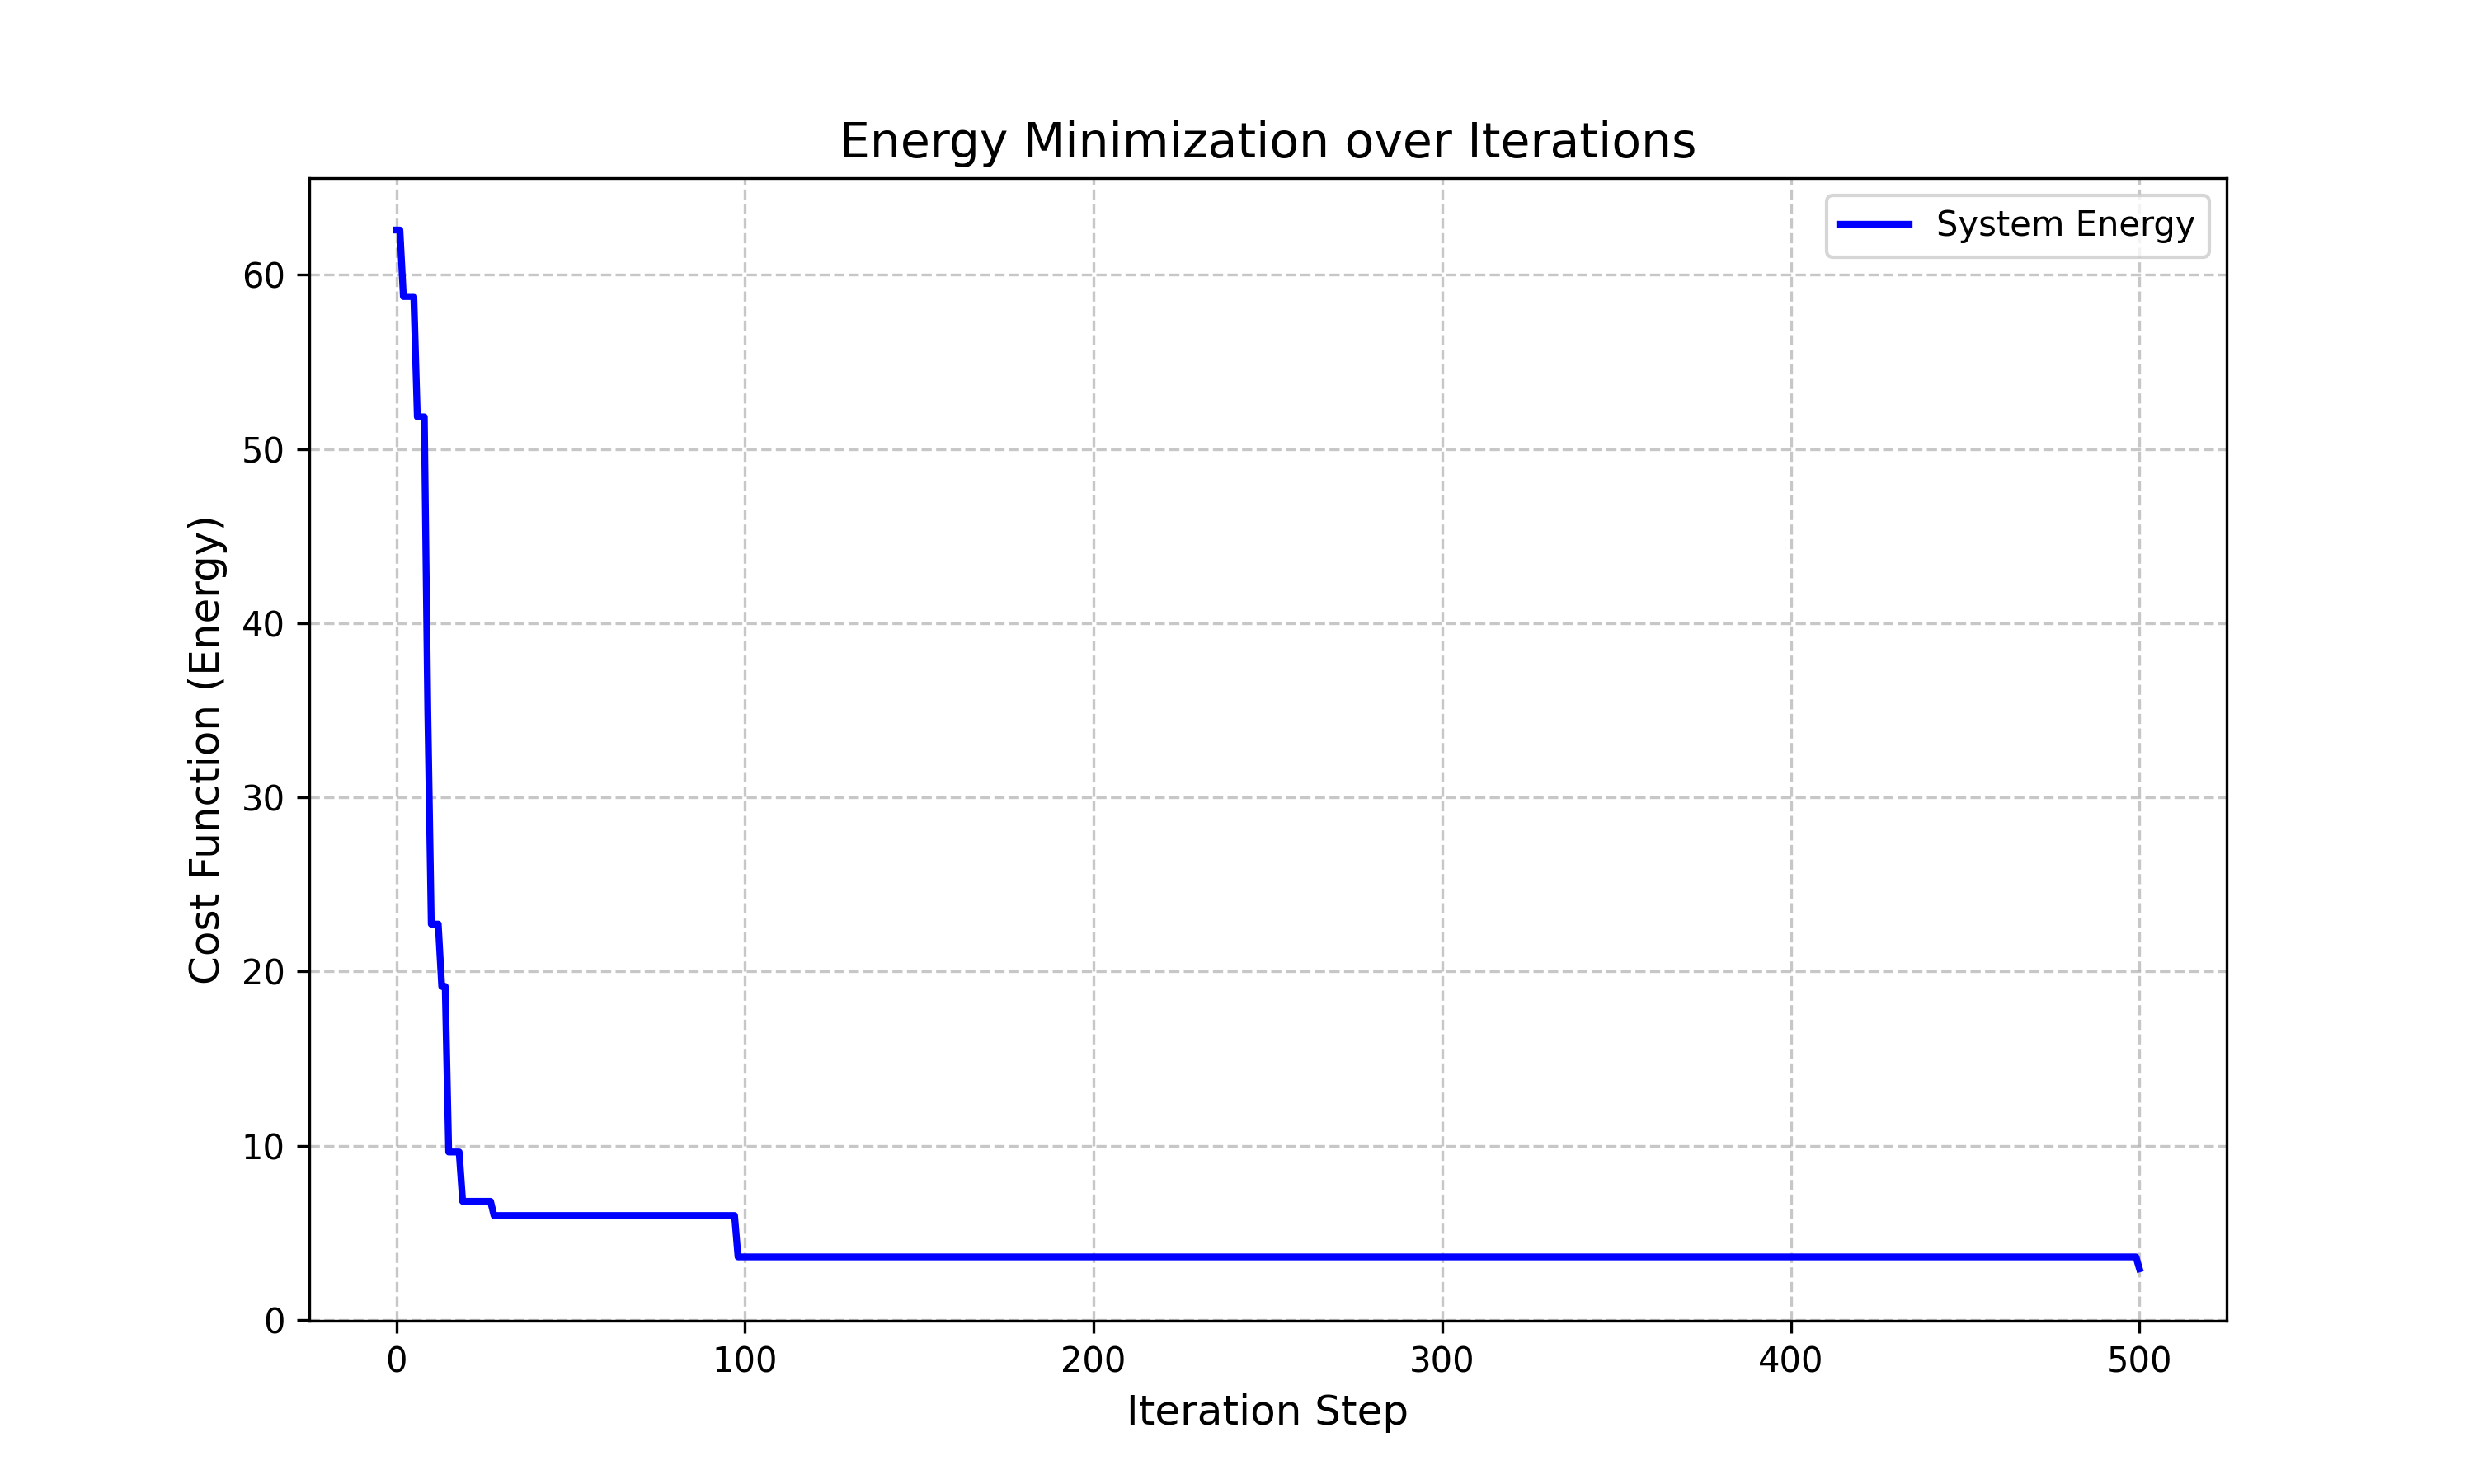
\includegraphics[width=0.45\textwidth]{../../docs/energy_plot.png}
    \caption{Energy landscape traversal during the optimization process. The plot shows the rapid convergence of the cost function (Euclidean distance between target and detected intensity) as the Simulated Annealing algorithm iteratively adjusts the spin configuration. The system successfully escapes local minima to reach a ground-state-like solution.}
    \label{fig:energy_plot}
\end{figure}

The results confirm that the optical interference reliably reproduces the Fourier transform $E(\mathbf{x}) \xrightarrow{\mathcal{F}} \tilde{E}(\mathbf{k})$, validating the physics engine at the core of the solver.

\subsection{Scalability and Performance}
The effective coupling matrix $J_{ij}$ in this system is all-to-all, limited only by the resolution of the SLM and the dynamic range of the camera. Current commercial SLMs ($>1920 \times 1080$ pixels) theoretically allow for systems with millions of spins, far exceeding the connectivity graphs of superconducting qubits. The time complexity for calculating the energy of a configuration is $O(1)$ in the optical domain (speed of light transit), whereas the digital feedback loop scales with the readout frame rate. This hybrid optical-digital approach offers a path to solving problems previously deemed intractable.
